\documentclass{article} % For LaTeX2e
\usepackage{nips2013submit_e,times}
\usepackage{hyperref}
\usepackage{url}
\usepackage{graphicx}
\usepackage{amsmath}
\usepackage{caption}
\usepackage{subcaption}
\usepackage{color}
%\documentstyle[nips2013submit_09,times,art10]{article} % For LaTeX 2.09


\title{10-601b: Mid-term report}


\author{
David S.~Hippocampus\thanks{ Use footnote for providing further information
about author (webpage, alternative address)---\emph{not} for acknowledging
funding agencies.} \\
Department of Computer Science\\
Cranberry-Lemon University\\
Pittsburgh, PA 15213 \\
\texttt{hippo@cs.cranberry-lemon.edu} \\
\And
Coauthor \\
Affiliation \\
Address \\
\texttt{email} \\
\AND
Coauthor \\
Affiliation \\
Address \\
\texttt{email} \\
\And
Coauthor \\
Affiliation \\
Address \\
\texttt{email} \\
\And
Coauthor \\
Affiliation \\
Address \\
\texttt{email} \\
(if needed)\\
}

% The \author macro works with any number of authors. There are two commands
% used to separate the names and addresses of multiple authors: \And and \AND.
%
% Using \And between authors leaves it to \LaTeX{} to determine where to break
% the lines. Using \AND forces a linebreak at that point. So, if \LaTeX{}
% puts 3 of 4 authors names on the first line, and the last on the second
% line, try using \AND instead of \And before the third author name.

\newcommand{\fix}{\marginpar{FIX}}
\newcommand{\new}{\marginpar{NEW}}

%\nipsfinalcopy % Uncomment for camera-ready version

\begin{document}


\maketitle

\begin{abstract}
    In this report, we list the results we've achieved for classifying the subset of the CIFAR-10 dataset. We use the K-nearest neighbours and SVM to achieve an accuracy of X\% and Y\% respectively. We also describe the approaches we have used to achieve these.\\
\end{abstract}

\section{Introduction}
    \begin{itemize}
        \item The problem statement
        \item The Cifar-10 dataset
        \item Our approaches
    \end{itemize}

\section{Exploratory data analysis}
    Before starting with the machine learning techniques, we tried to understand the dataset we were provided. We have been provided with a subset of the CIFAR-10 dataset. We looked that the \textbf{distribution of training labels} provided to us. This was to ensure the training samples are not skewed towards a certain label. We found that `airplane` class had the least number of training samples (about 470) and `frog` class had the maximum (about 520). The difference is minimal and should not affect training.\\

    We looked at the \textbf{colour distribution} in the overall training dataset and the colour distribution in individual classes. The images seem to follow a normal distribution around different means and have different variances for the red, green and blue components. This was expected and should not affect training of our algorithms at all.\\

    Finally, we constructed the \textbf{average image of each class}. This was to look for specific patterns that might exist in the dataset. Any sharp patterns in the average image would skew training performance. However, we did not find any such patterns with the given dataset.\\

    \textbf{Can we find the average HOG for each class?}
    \begin{figure}[h]
        \centering
        \begin{subfigure}{.2\linewidth}
            \centering
            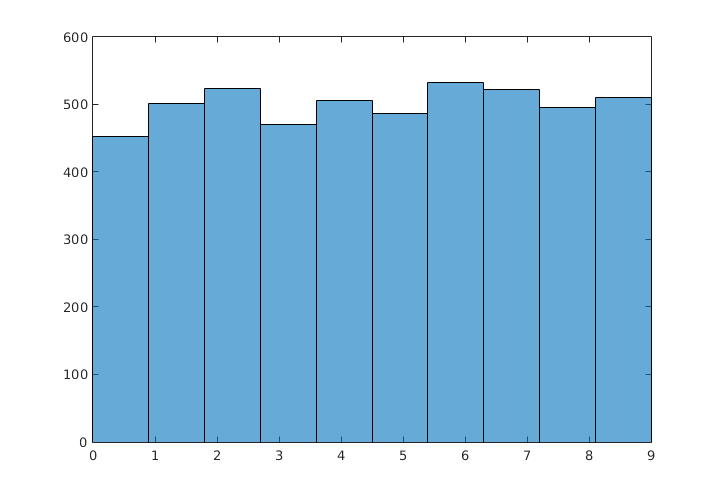
\includegraphics[width=.75\linewidth]{label-distribution.png}
        \caption{Distribution of the ground truth labels}
        \end{subfigure}
        \begin{subfigure}{.2\linewidth}
            \centering
            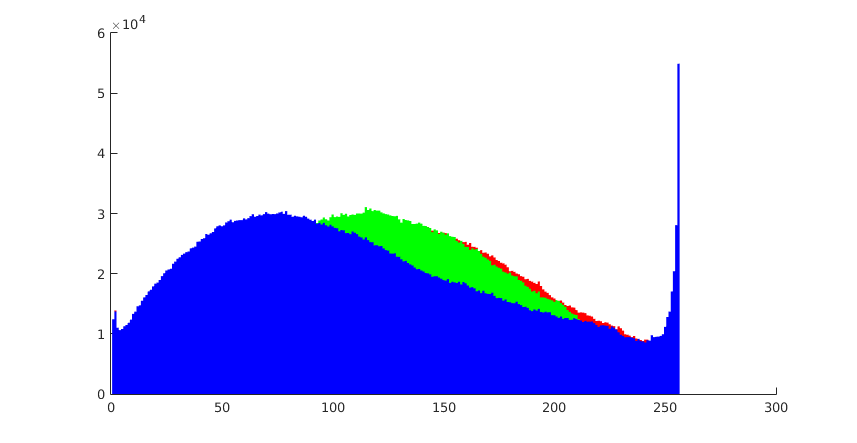
\includegraphics[width=\linewidth]{hist-overall.png}
        \caption{Distribution of RGB across all images}
        \end{subfigure}
        \begin{subfigure}{.2\linewidth}
            \centering
            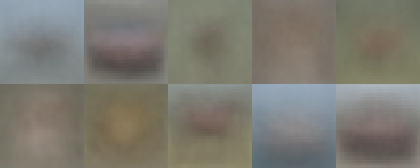
\includegraphics[width=\linewidth]{avg-img.png}
        \caption{The average image for each class}
        \end{subfigure}
        \begin{subfigure}{.2\linewidth}
            \centering
            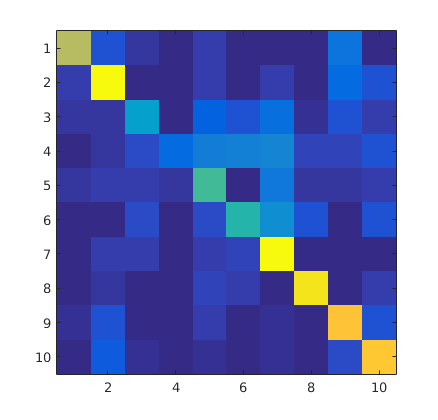
\includegraphics[width=.5\linewidth]{knn-confusion.png}
            \caption{Confusion matrix for k-NN}
        \end{subfigure}
        \caption{}
    \end{figure}
    \begin{figure}[h]
        \begin{subfigure}{\linewidth}
            \centering
            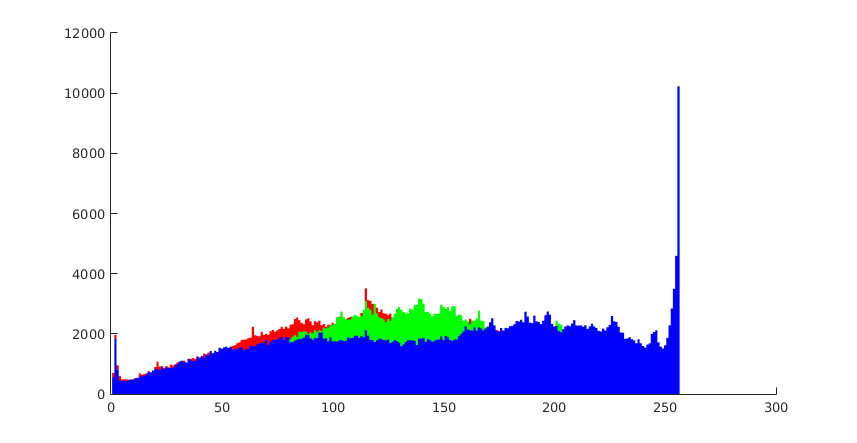
\includegraphics[width=.18\linewidth]{hist-class-0.png}
            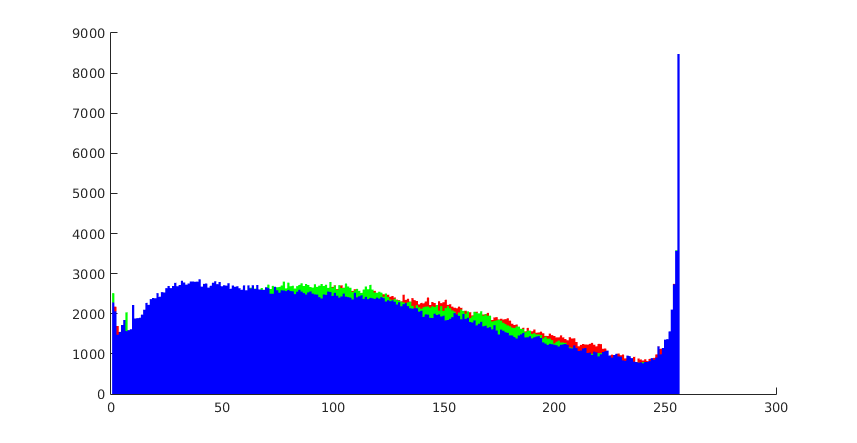
\includegraphics[width=.18\linewidth]{hist-class-1.png}
            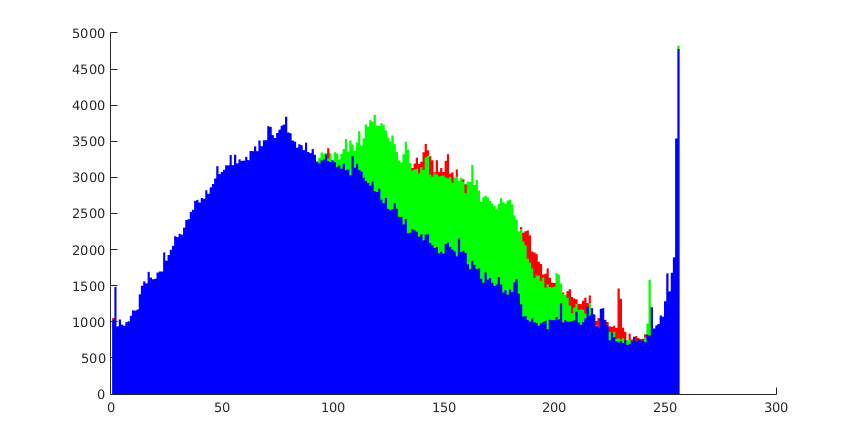
\includegraphics[width=.18\linewidth]{hist-class-2.png}
            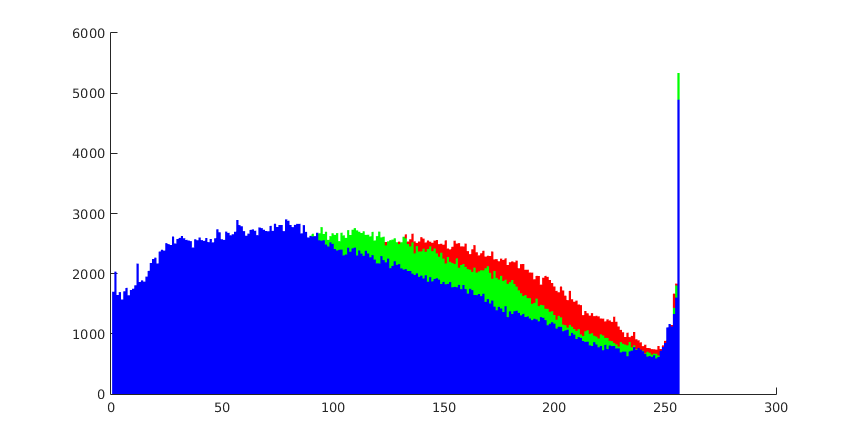
\includegraphics[width=.18\linewidth]{hist-class-3.png}
            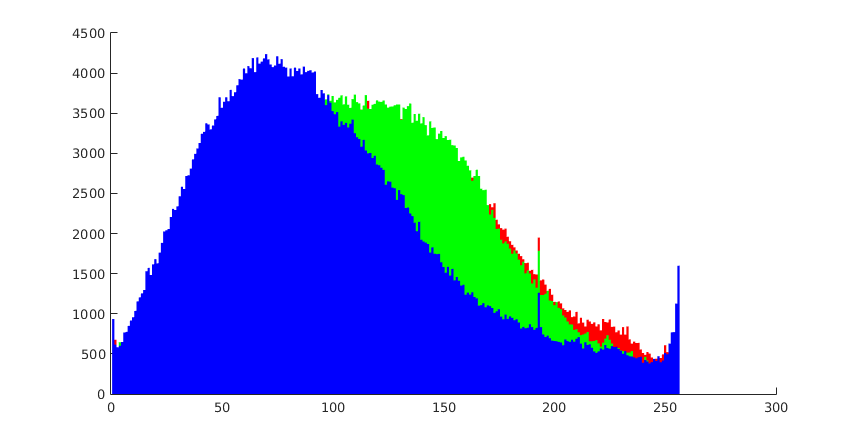
\includegraphics[width=.18\linewidth]{hist-class-4.png}
        \end{subfigure}
        \begin{subfigure}{\linewidth}
            \centering
            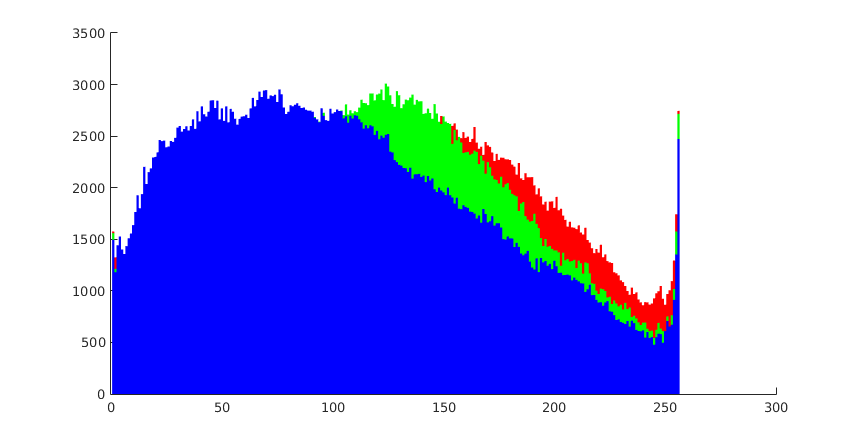
\includegraphics[width=.18\linewidth]{hist-class-5.png}
            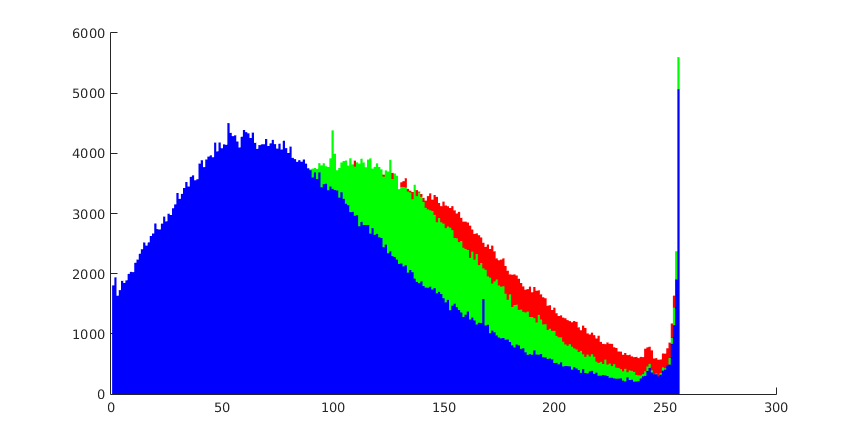
\includegraphics[width=.18\linewidth]{hist-class-6.png}
            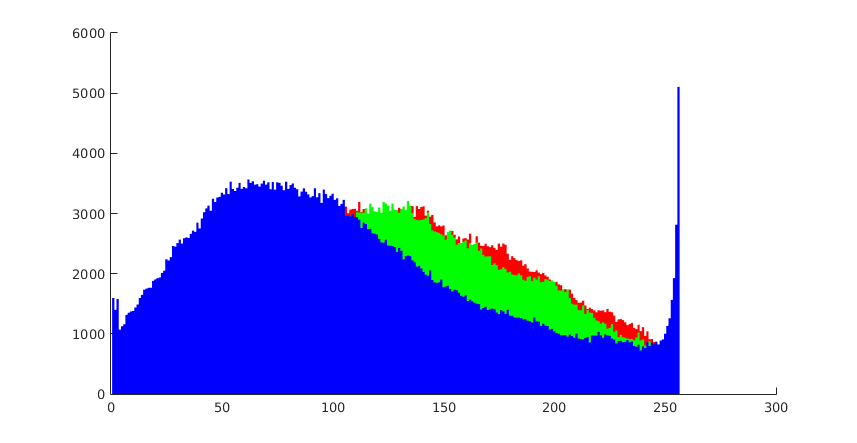
\includegraphics[width=.18\linewidth]{hist-class-7.png}
            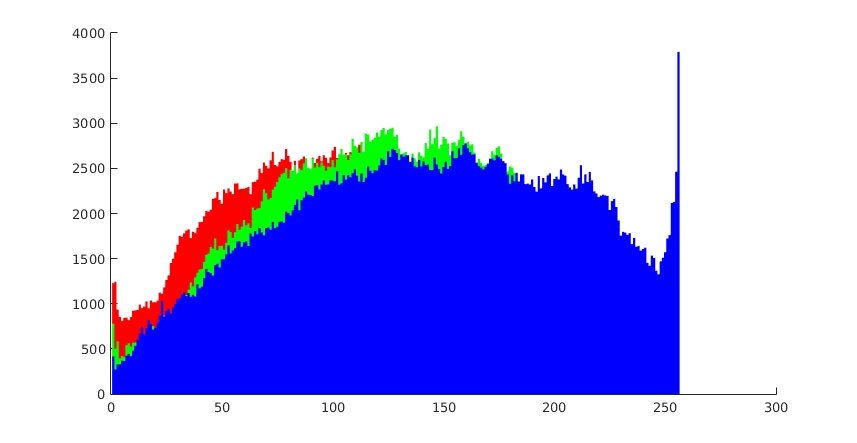
\includegraphics[width=.18\linewidth]{hist-class-8.png}
            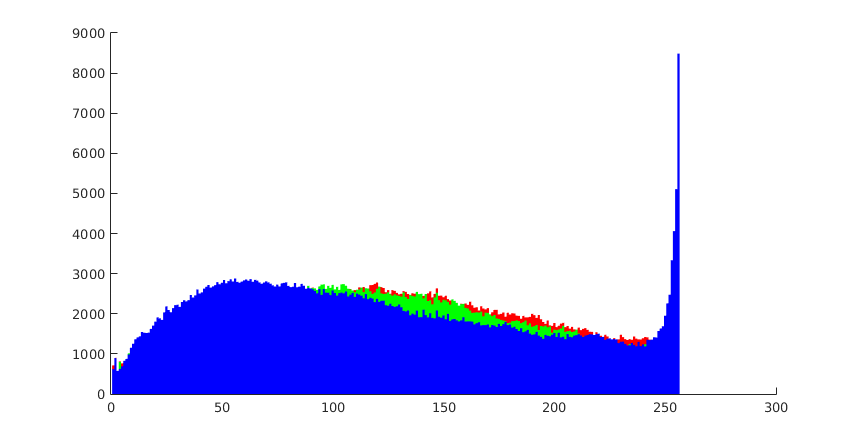
\includegraphics[width=.18\linewidth]{hist-class-9.png}
        \end{subfigure}
        \caption{RGB histogram for each class}
    \end{figure}
    

\section{Classification with K-means and K-Nearest Neighbours}
    The very first approach we tried was using the simple k-means and k-nearest neighbours approaches. These are simple to implement and help understand the dataset provided to use better. Details of problems with these techniques are provided in detail below.\\
    \subsection{K-Means} % (fold)
        The K-means clustering algorithm was the first technique we tried. The first attempt was to use the raw image data and find clusters in the pixel RGB values. This approach took a long to train and produced bad results. With a constant classifier (one that always returns a particular class), we would have about 10\% accuracy. We achieved about 15.3\% accuracy with the naive K-means classifier. This improvement is very small compared to the effort required for the code.\\

        The next attempt was to cluster responses from a filter bank. We used two sets of filter banks - regular filters and \textbf{Gabor filters}. The training time for this increased further but produced a very tiny increase in accuracy (about 16.7\%). \\

        Given the training time required for K-means and the accuracy, we decided to try K-nearest neighbours. The voting algorithm would be robust to noise in the training inputs.\\
    % subsubsection K-Means (end)

    %%%%%%%%%%%%%%%%%%%%%%%%%%%%%%%%%%%%%%%%%%
    \subsection{K-Nearest Neighbours} % (fold)
        We used the K-nearest neighbours on three different feature spaces. The first was raw images. The accuracy was almost as good as the K-means classifier.\\
        
        Second, we tried passing images through the filter bank and Gabor filters used in the previous section. The results were better than K-means (~29\%). This increase in accuracy can be attributed to the classifier being robust when the input training samples are noisy. We used $K=51$ to achieve this result.\\

        To improve accuracy further, we calculated the Histogram of Gradients features on the image and used those for classification. This improved the accuracy to ~53\%. The improvement was because certain classes in the image can be represented accurately with orientation histograms (cars, for example).\\

        \textbf{Talk about the confusion matrix}
        \textbf{Talk about the classes that fail}
    % subsection K-Nearest Neighbours (end)

    %%%%%%%%%%%%%%%%%%%%%%%%%%%%%%%%%%%%%%%%%%
    \subsection{Results} % (fold)
        Upon analysing the confusion matrix for K-Nearest neighbours (Figure 1 (d)), we found that the perfectly classified labels belonged to classes with several sharp and well defined edges - cars, airplanes, ships, trucks. The horse and frog classes seem to perform quite well too - however, the bird, cat, deer and dog classes are harder to classify.\\

        From this, we can infer why the classifier fails. At such low resolutions, the HOG features are unable to capture the distinctive features of these classes. Most of them seem to be mammals with 4 legs and thus the confusion. Using HOG with higher resolutions (with smaller cell sizes), we found that accuracy of the classifier decreased to below 50\% with no increase in accuracy on the problematic classes.\\
        % TABLE SAMPLE
        \begin{table}[t]
            \caption{Results with K-means clustering and K-nearest neighbours}
            \begin{center}
                \begin{tabular}{lll}
                    \multicolumn{1}{c}{\bf Technique} &\multicolumn{1}{c}{\bf Training time} &\multicolumn{1}{c}{\bf Accuracy}\\
                    \\ \hline \\
                    Constant classifier & 0 sec & 8-11\%\\
                    K-means (pixels) & 20-30 min & 15.3\% \\
                    K-means (filter bank) & 1 hour& 16.5\% \\
                    K-means (Gabor filters) &1-1.5 hours & 16.7\% \\
                    K-Nearest (pixels) & 5-10 seconds & 16.4\% \\
                    K-Nearest (filter bank) &1 minute& 28.6\% \\
                    K-Nearest (Gabor filters) &1 minute& 29.4\% \\
                    K-Nearest (HOGs) &1 minute& 53.1\% \\
                \end{tabular}
            \end{center}
        \end{table}

    % subsection Results (end)

\section{Support vector machines}
    \begin{itemize}
        \item The outline goes here?
        \item More outline here
    \end{itemize}

    %%%%%%%%%%%%%%%%%%%%%%%%%%%%%%%%%%%%%%%%%%
    \subsection{Results} % (fold)
    \label{sub:Results}
    
    % subsection Results (end)

% FIGURE SAMPLE
\begin{figure}[h]
    \begin{center}
    %\framebox[4.0in]{$\;$}
    \fbox{\rule[-.5cm]{0cm}{4cm} \rule[-.5cm]{4cm}{0cm}}
    \end{center}
    \caption{Sample figure caption.}
\end{figure}

% TABLE SAMPLE
\begin{table}[t]
    \caption{Sample table title}
    \begin{center}
        \begin{tabular}{ll}
        \multicolumn{1}{c}{\bf PART}  &\multicolumn{1}{c}{\bf DESCRIPTION}
        \\ \hline \\
        Dendrite         &Input terminal \\
        Axon             &Output terminal \\
        Soma             &Cell body (contains cell nucleus) \\
        \end{tabular}
    \end{center}
\end{table}

\section{Future work}
    Until now, we have achieved a maximum accuracy of XYZ\%. We have used simple techniques like k-means, k-nearest and more sophisticated techniques like SVM. Our next trial will be with a discriminative sum-product networks. The paper claims to achieve a high accuracy using a network approach and using gradient descent.

\subsubsection*{References}

\small{
    [1] Robert Gens, et al (2012) Discriminative learning of sum-product networks {\it Neural Information Processing Systems}

[2] Alexander, J.A. \& Mozer, M.C. (1995) Template-based algorithms
for connectionist rule extraction. In G. Tesauro, D. S. Touretzky
and T.K. Leen (eds.), {\it Advances in Neural Information Processing
Systems 7}, pp. 609-616. Cambridge, MA: MIT Press.

[3] Bower, J.M. \& Beeman, D. (1995) {\it The Book of GENESIS: Exploring
Realistic Neural Models with the GEneral NEural SImulation System.}
New York: TELOS/Springer-Verlag.

[4] Hasselmo, M.E., Schnell, E. \& Barkai, E. (1995) Dynamics of learning
and recall at excitatory recurrent synapses and cholinergic modulation
in rat hippocampal region CA3. {\it Journal of Neuroscience}
{\bf 15}(7):5249-5262.
}

\end{document}
